%%-----------------Document Type----------------------------------
\documentclass[a4paper,11pt]{article}
\usepackage[utf8]{inputenc}
\usepackage[left=2cm, text={17cm,24cm}, top=3cm]{geometry}
\usepackage{times}
\usepackage[czech]{babel}
\usepackage{pdflscape}
\usepackage[ruled,czech,linesnumbered,longend,noline]{algorithm2e}
\usepackage{graphics}
\usepackage{multirow}
\newcommand\quot[1]{\quotedblbase #1\textquotedblleft}

\begin{document}
	%%-----------------Title------------------------------------------
	\begin{center}
		\Huge
		\textsc{\Huge{Vysoké učení technické v~Brně}\\
			\huge{Fakulta informačních technologií}}\\
		\vspace{\stretch{0.382}}
		\Large{Typografie a publikování - 3. projekt}\\
		\Huge{Tabulky a obrázky}\vspace{\stretch{0.618}}
	\end{center}
	\thispagestyle{empty}
	\normalsize{\today \hfill Jozef Urbanovský}
	\newpage
	
	\pagenumbering{arabic}
	\setcounter{page}{1}
	\section{Úvodní strana}\label{section:1}
	Název práce umístěte do zlatého řezu a nezapomeňte uvést dnešní datum a vaše jméno a přijmení.
	
	\section{Tabulky}\label{section:2}
	Pro sázení tabulek můžeme použít buď prostředí \texttt{tabbing} nebo prostředí \texttt{tabular}.
	
	\subsection{Prostředí \texttt{tabbing}}
	Při použití \texttt{tabbing} vypadá tabulka následovně:
	\begin{tabbing}
		\hspace*{3cm}\=\hspace*{1.5cm}\= \kill
		\textbf{Ovoce} \> \textbf{Cena} \> \textbf{Množství} \\
		Jablka \> 25,90 \> 3 kg\\
		Hrušky \> 27,40 \>2,5 kg\\
		Vodní melouny \> 35,-- \> 1 kus
	\end{tabbing}
	\bigskip
	
	\noindent Toto prostředí se dá také použít pro sázení algoritmů, ovšem vhodnější je použít 
	prostředí \texttt{algorithm} nebo \texttt{algorithm2e} (viz sekce \ref{section:3}).
	
	\subsection{Prostředí tabular}
	Další možností, jak vytvořit tabulku, je použít prostředí \texttt{tabular}. 
	Tabulky pak budou vypadat takto
	\footnote{Kdyby byl problem s~\texttt{cline}, zkuste se podívat třeba sem: 
		http://www.abclinuxu.cz/tex/poradna/show/325037 \vspace{\fill}}
	\bigskip
	
	
	\begin{table}[ht]
		\begin{center}
			\catcode`\-=12
			\begin{tabular}{ |l|c|c| } 
				\hline
				&\multicolumn{2}{c|}{\textbf{Cena}}\\ \cline{2-3}
				\textbf{Měna} & \textbf{nákup} & \textbf{prodej}\\
				\hline
				EUR & 27,02 & 27,20 \\ 
				GBP & 31,08 & 31,80 \\ 
				USD & 25,15 & 25,51 \\ 
				\hline
			\end{tabular}
			\caption{Tabulka kurzů k~dnešnímu dni}
			\label{tab:tabulka1}
		\end{center}
	\end{table}
	
	\begin{table}[ht]
		\catcode`\-=12	
		\begin{center}
			\begin{tabular}{|c|c|} 
				\hline
				$A$ & $\neg A$\\
				\hline
				
				\textbf{P} & N \\ 
				\textbf{O} & O \\ 
				\textbf{X} & X \\ 
				\textbf{N} & P \\
				
				\hline
			\end{tabular}
			%
			\begin{tabular}{|c|c|c|c|c|c|}
				\hline
				
				\multicolumn{2}{|c|}{\multirow{2}{*}{$A \land B$}}&\multicolumn{4}{c|}{$B$}\\ \cline{3-6}
				\multicolumn{2}{|c|}{}&\textbf{P} & \textbf{O} & \textbf{X} & \textbf{N}\\ \hline
				{\multirow{4}{*}{$A$}}
				& \textbf{P} & P & O & X & N\\ \cline{2-6}
				& \textbf{O} & O & O & N & N\\ \cline{2-6}
				& \textbf{X} & X & N & X & N\\ \cline{2-6}
				& \textbf{N} & N & N & N & N\\ 
				
				\hline
			\end{tabular}
			%
			\begin{tabular}{|c|c|c|c|c|c|}
				\hline
				
				\multicolumn{2}{|c|}{\multirow{2}{*}{$A \lor B$}}&\multicolumn{4}{c|}{$B$}\\ \cline{3-6}
				\multicolumn{2}{|c|}{}&\textbf{P} & \textbf{O} & \textbf{X} & \textbf{N}\\ \hline
				{\multirow{4}{*}{$A$}}& \textbf{P} & P & P & P & P\\\cline{2-6}
				& \textbf{O} & P & O & P & O\\ \cline{2-6}
				& \textbf{X} & P & P & X & X\\ \cline{2-6}
				& \textbf{N} & P & O & X & N\\ 
				
				\hline
			\end{tabular}
			%
			\begin{tabular}{|c|c|c|c|c|c|}
				\hline
				
				\multicolumn{2}{|c|}{\multirow{2}{*}{$A \rightarrow B$}}&\multicolumn{4}{c|}{$B$}\\ \cline{3-6}
				\multicolumn{2}{|c|}{}&\textbf{P} & \textbf{O} & \textbf{X} & \textbf{N}\\ \hline
				{\multirow{4}{*}{$A$}}& \textbf{P} & P & O & X & N\\ \cline{2-6}
				& \textbf{O} & P & O & P & O\\ \cline{2-6}
				& \textbf{X} & P & P & X & X\\ \cline{2-6}
				& \textbf{N} & P & P & P & P\\
				\hline
			\end{tabular}
		
			\caption{Protože Kleeneho trojhodnotová logika už je  \quot{zastaralá}, uvádíme si zde příklad čtyřhodnotové logiky}
			
			\label{tab:tabulka2}
		\end{center}
	\end{table} 
	\bigskip
	
	\newpage
	
	\section{Algoritmy}\label{section:3}
	
	\noindent Pokud budeme chtít vysázet algoritmus, můžeme použít prostředí 
	\texttt{ algorithm}
	\footnote{Pro nápovědu, jak zacházet s~prostředím 
		\texttt{algorithm}, můžeme zkusit tuhle stránku:\\ http://ftp.cstug.cz/pub/tex/CTAN/macros/latex/contrib/algorithms/algorithms.pdf.} nebo \texttt{ algorithm2e}
	\footnote{Pro \texttt{algorithm2e} zase tuhle: http://ftp.cstug.cz/pub/tex/CTAN/macros/latex/contrib/algorithm2e/doc/algorithm2e.pdf}. 
	Příklad použití prostředí \texttt{ algorithm2e} viz Algoritmus 1.\\
	
	
	\begin{algorithm}[H]
		\label{algoritmus1} 
		\SetKwInOut{Input}{Input}\SetKwInOut{Output}{Output}
		\SetNlSty{}{}{:}
		\Input{$(X_{t-1}, u_t, z_t)$}
		\Output{$X_t$}
		\medskip 
		\SetNlSkip{-1em}
		\Indp\Indpp
		$\overline{X_t}=X_t=0$\\
		\For{$k = 1$ \textup{to} $M$}
		{
			$x_t^{[k]}=$ \textit{sample\_motion\_model}$(u_t,x_{t-1}^{[k]})$\\
			$\omega_t^{[k]} =$ \textit{measurement\_model}$(z_t,x_t^{[k]},m_{t-1})$\\
			$m_t^{[k]}=$ \textit{updated\_occupancy\_grid}$(z_t,x_t^{[k]},m_{t-1}^{[k]})$\\
			$\overline{X_t} = \overline{X_t}\ +\ \langle x_x^{[m]}, \omega_t^{[m]}\rangle$
		}
		\For{$k = 1$ \textup{to} $M$}
		{
			draw $i$ with probability $\approx \omega_t^{[i]}$ \\
			add $\langle x_x^{[k]}, m_t^{[k]}\rangle$ to $X_t$
		}
		\KwRet{$X_t$}
		\caption{\textsc{FastSLAM}}
		\label{algoritmus1}
	\end{algorithm}
	\bigskip
	
	
	
	\section{Obrázky}\label{section:4}
	\noindent Do našich článků můžeme samozřejmě vkládat obrázky. Pokud je obrázkem fotografie, můžeme klidně použít bitmapový soubor. Pokud by to ale mělo být nějaké schéma nebo něco podobného, je dobrým zvykem takovýto obrázek vytvořit vektorově.\par
	\begin{figure}[ht]
		\begin{center}
			\scalebox{0.4}
			{
				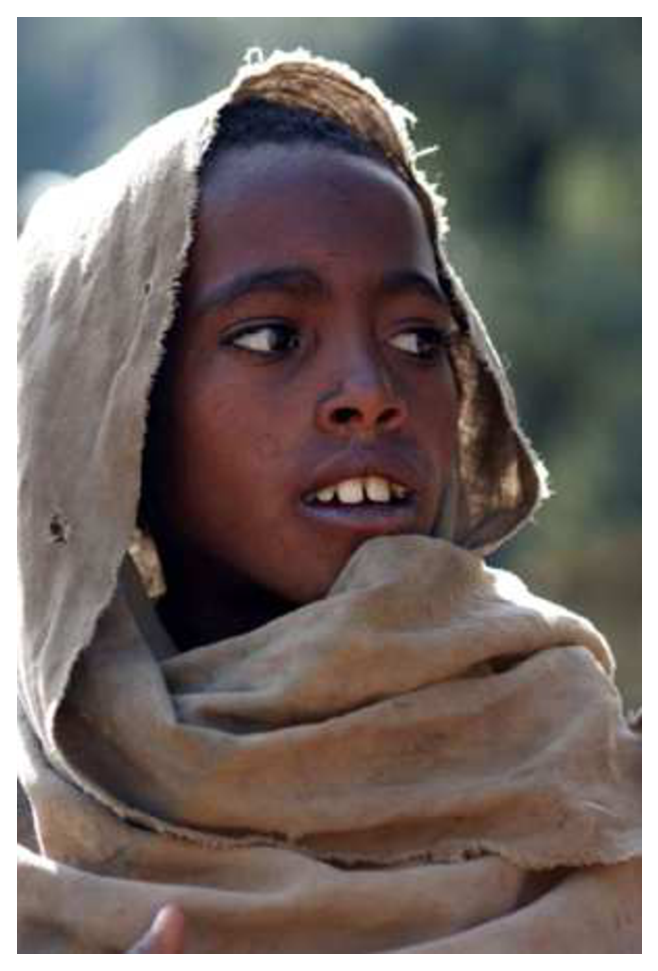
\includegraphics{etiopan.eps}
				\reflectbox{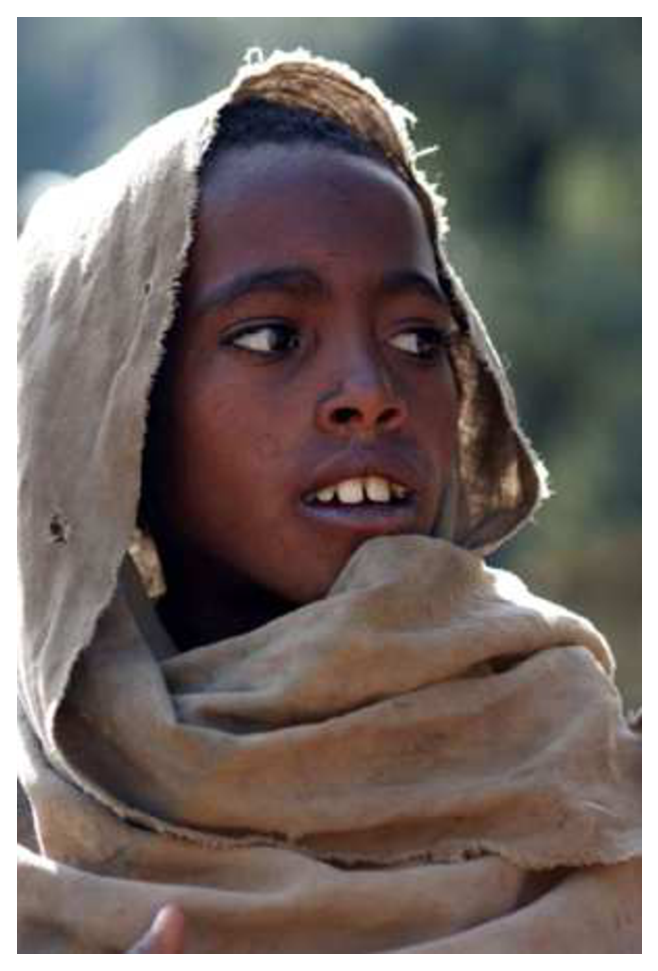
\includegraphics{etiopan.eps}}
			}
			\caption{Malý etiopánek a jeho bratříček}
			\label{obrazok1}
		\end{center}
	\end{figure}
	
	
	\newpage
	Rozdíl mezi vektorovým\,\dots
	\begin{figure}[ht]
		\begin{center}
			\scalebox{0.4}{
\includegraphics{oniisan.eps}}
			\caption{Vektorový obrázek}
			\label{obrazok2}
		\end{center}
	\end{figure}\\
	\dots\,a bitmapovým obrázkem
	
	\begin{figure}[ht]
		\begin{center}
			\scalebox{0.6}{
\includegraphics{oniisan2.eps}}
			\caption{Bitmapový obrázek}
			\label{obrazok3}
		\end{center}
	\end{figure} 
	\noindent se projeví například při zvětšení.\par
	Odkazy (nejen ty) na obrázky \ref{obrazok1},
	\ref{obrazok2} a \ref{obrazok3}, na tabulky \ref{tab:tabulka1} a \ref{tab:tabulka2} a také na algoritmus \ref{algoritmus1} jsou udělány pomocí křížových odkazů. Pak je ovšem potřeba zdrojový soubor přeložit dvakrát.\par
	Vektorové obrázky lze vytvořit i přímo v~\LaTeX u, například pomocí prostředí \texttt{picture.}
	\newpage
	
	
	\begin{landscape}
		\begin{figure}[ht]
			\centering
			\setlength{\unitlength}{1cm}
			\begin{picture}(21,11)
			
			%base
			\linethickness{4pt}
			\put(0.5,1.5){\line(1,0){20.2}}
			
			\linethickness{1.5pt}
			\put(0,0){\framebox(21,11){}}
			
			\put(17,8.5){\circle{1.4}}
			
			%horizontal lines from base
			\put(2,5.5){\line(0,-1){4}} 
			\put(3,3){\line(0,-1){1.5}}
			\put(19,2.5){\line(0,-1){1}}
			
			%vertical lines from base
			\put(2,5.5){\line(1,0){5}} 
			\put(3,3){\line(1,0){4.5}}
			\put(9,2.5){\line(1,0){10}}
			
			%left right level 0
			\put(8,3.8){\line(1,0){10.82}}
			\put(18.8,3.8){\line(0,-1){1.3}}
			\put(8,3.8){\line(0,-1){0.95}}
			
			%left right level 1
			\put(4,4.8){\line(1,0){15}}
			\put(4,4){\line(1,0){15}}
			\put(19,4.8){\line(0,-1){0.8}}
			\put(4,4.8){\line(0,-1){0.8}}
			
			%top level
			\put(7,6){\line(1,0){6}}
			\put(13,6){\line(0,-1){1.2}}
			\put(7,6){\line(0,-1){1.2}}
			
			%left right level 2
			\put(13,5){\line(1,0){5.02}}
			\put(18,5){\line(0,-1){0.2}}
			
			%oblique lines
			\thicklines
			\put(7.5,3){\line(3,-1){4.5}}
			\put(4,4){\line(3,-2){1.5}}
			
			\end{picture}
			\caption{Vektorový obrázek.}
		\end{figure}
	\end{landscape}
	
	
\end{document} 


